\documentclass[t, pdftex]{beamer}
\usetheme[]{Cockrell}
%\usetheme[dept=Mechanical\ Engineering]{cockrell}

% \useoutertheme[subsection=false]{miniframes}
% \useoutertheme[footline=authortitle]{miniframes}
% \setbeamercolor{mini frame}{fg=white,bg=utblack}
%\usepackage{etoolbox}
%\patchcmd{\sectionentry}{\usebeamercolor[fg]{section in head/foot}}{\usebeamercolor[fg]{mini frame}}{}{}

\mode<presentation> {	
	% The Beamer class comes with a number of default slide themes	
	% which change the colors and layouts of slides. Below this is a list	
	% of all the themes, uncomment each in turn to see what they look like.
	
		
	%\usetheme{default}	
	%\usetheme{AnnArbor}	
	%\usetheme{Antibes}	
	%\usetheme{Bergen}	
	%\usetheme{Berkeley}	
	%\usetheme{Berlin}	
	%\usetheme{Boadilla}	
	%\usetheme{CambridgeUS}	
	%\usetheme{Copenhagen}	
	%\usetheme{Darmstadt}	
	%\usetheme{Dresden}	
	%\usetheme{Frankfurt}	
	%\usetheme{Goettingen}	
	%\usetheme{Hannover}	
	%\usetheme{Ilmenau}	
	%\usetheme{JuanLesPins}	
	%\usetheme{Luebeck}	
	%\usetheme{Madrid}	
	%\usetheme{Malmoe}	
	%\usetheme{Marburg}	
	%\usetheme{Montpellier}	
	%\usetheme{PaloAlto}	
	%\usetheme{Pittsburgh}	
	%\usetheme{Rochester}	
	%\usetheme{Singapore}	
	%\usetheme{Szeged}	
	%\usetheme{Warsaw}	
	
	% As well as themes, the Beamer class has a number of color themes	
	% for any slide theme. Uncomment each of these in turn to see how it	
	% changes the colors of your current slide theme.
	
	%\usecolortheme{albatross}	
	%\usecolortheme{beaver}	
	%\usecolortheme{beetle}	
	%\usecolortheme{crane}	
	%\usecolortheme{dolphin}	
	\usecolortheme{dove}	
	%\usecolortheme{fly}	
	%\usecolortheme{lily}	
	%\usecolortheme{orchid}	
	%\usecolortheme{rose}	
	%\usecolortheme{seagull}	
	%\usecolortheme{seahorse}	
	%\usecolortheme{whale}	
	%\usecolortheme{wolverine}
	
		
	\setbeamertemplate{footline} % To remove the footer line in all slides uncomment this line	
	%\setbeamertemplate{footline}[page number] % To replace the footer line in all slides with a simple slide count uncomment this line	
	
	%\setbeamertemplate{navigation symbols}{} % To remove the navigation symbols from the bottom of all slides uncomment this line
    
    \setbeamertemplate{itemize item}{\color{utblack}$\blacktriangleright$}
}

% Additional Packages
%\usepackage{etex}
%\usepackage[bigfiles]{media9}
%\graphicspath{{./figs/}}

%Enable cancelto in math
\usepackage{color}
\usepackage{cancel}
\usepackage[]{algorithm2e}
\usepackage{mathtools}
\usepackage{amsmath}
\usepackage{pgfgantt}
\usepackage[version=3]{mhchem} % Package for chemical equation typesetting \ce{}
\usepackage{siunitx} % Provides the \SI{}{} and \si{}
%\usepackage[font=scriptsize,justification=centering]{caption}
\renewcommand{\CancelColor}{\color{utorange}}
\DeclareMathOperator*{\E}{\mathbb{E}}
\bibliography{example.bib}


\title{A CFD-Informed Hi2Low Method for Improving Subchannel Resolution Crud Predictions}
\subtitle{}
\author{William Gurecky}
\date{\today}


\begin{document}
\setbeamertemplate{caption}{\raggedright\insertcaption\par}
\setbeamertemplate{caption}{%
\begin{beamercolorbox}[wd=.5\paperwidth, sep=.2ex]{block body}\insertcaption%
\end{beamercolorbox}%
}

% =========================================================================== %
\titleframe
\frame{\frametitle{Outline}\tableofcontents}

% =========================================================================== %
\section{Introduction}
\subsection*{Crud Background}
\begin{frame}
    \frametitle{Chalk River Unidentified Deposit (crud)}
    Crud forms a porous layer on the surface of fuel rods.  It is primarily comprised of Nickel Ferrite.
\begin{small}
    \begin{itemize}
    \item Preferentially deposited where temperature is high - near or above saturation point - and where local shear stresses on the rod are low.
	\item CRUD induced local corrosion (CILC).
    \item CRUD induced power shift (CIPS). Also known as axial offset anomaly (AOA).
    \begin{itemize} 
    	\item CRUD and tends to uptake and retain boron from the coolant.
    	\item \ce{Li^+} + \ce{B(OH)_3}   $\rightarrow$ \ce{LiBO_2} + \ce{H^+} + \ce{H_2O} .
    \end{itemize}
    \item CASL developed CRUD simulation package, MAMBA, which is integrated with the VERA core simulator providing.  Goal: provide a \emph{predictive} CIPS tool.
    \end{itemize}
\end{small}
%\begin{figure}[!htbp]
%\centering
%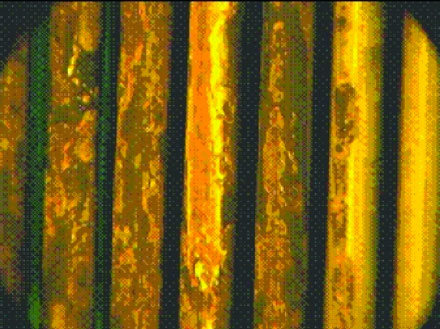
\includegraphics[width=4cm]{figs/crud-crud.jpg}
%\caption{CRUD on fuel rods.}
%\label{log_closed}
%\end{figure}
%
    \begin{figure}
        \centering
        \begin{minipage}{.7\textwidth}
            \centering
            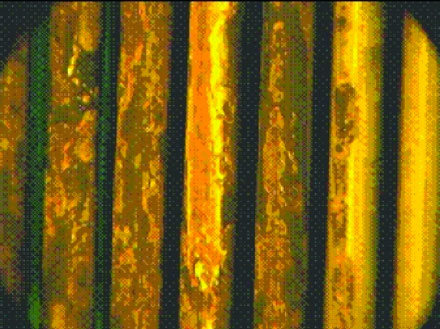
\includegraphics[width=6cm]{figs/crud-crud.jpg}
        \end{minipage}%
        \begin{minipage}{.4\textwidth}
            \centering
            \includegraphics[width=6cm]{figs/crud_flake_ex.png}
        \end{minipage}
    \end{figure}
\end{frame}

% =========================================================================== %
\subsection*{Motivation}
\begin{frame}
    \frametitle{Crud Induced Power Shift (CIPS)}
    \begin{figure}
        \centering
        \begin{minipage}{.5\textwidth}
            \centering
            \includegraphics[width=6cm]{figs/ao_mpact_ctf.png}
            \caption{Core averaged \% axial offset.  [CASL-I-2015-0318-000]}
        \end{minipage}%
        \begin{minipage}{.5\textwidth}
            \centering
            \includegraphics[width=6cm]{figs/core_b10_mpact_ctf.png}
            \caption{VERA WBNP1 Cycle 7 CRUD \ce{^{10}B}. \\ $@ 16.08 [MWD/MTU]$}
        \end{minipage}
    \end{figure}
\end{frame}

% =========================================================================== %
\subsection*{Motivation}
\begin{frame}
\frametitle{Current Crud Model Deficiencies}
\begin{itemize}
    \item \textbf{Incorrect boundary conditions provided to the crud code.}
    \begin{itemize}
        \item Fine scale flow details around spacer grids are not resolved by subchannel codes.  It is imperative for CILC analysis to capture the influence of the spacer grids on the crud deposition rate.  
        \item It is also important to account for the presence of spacer grids on crud growth when predicting CIPS.
    \end{itemize}
    \item Incorrect simulated crud chemistry, pore fill mechanisms, and intra-crud species transport models.
    \item Difficulty accounting for the source of corrosion products and nickel and iron particulate entrained in the primary coolant loop.
    \begin{itemize}
        \item Requires understanding of the metallurgy of all primary loop components. 
        \item Plants of different make and vintage require a predictive corrosion and erosion source term models.
    \end{itemize}
\end{itemize}
\end{frame}

% =========================================================================== %
\subsection*{High Fidelity Crud Simulation}
\begin{frame}[shrink=20]
    \frametitle{Coupled CFD/Crud Calculation}
    \begin{itemize}
    \item CFD/Crud coupling is useful for single-pin or single-assembly CRUD estimates.  Fine scale flow near spacer grid impacted surface crud distribution.  Important for quantifying crud induced local corrosion (CILC) risk.
    \item CFD/Crud simulations are too numerically costly for full core simulation.
    \end{itemize}
        \begin{figure}[!htbp]
\centering
\includegraphics[width=0.99\textwidth]{figs/combo_180x.png}
\label{log_closed}
    \end{figure}
\end{frame}

% =========================================================================== %
\subsection*{CFD and Subchannel Mesh Background}
\begin{frame}
Differences between CTF (subchannel) and CFD meshes for a single pin.
\begin{figure}
        \centering
        \begin{minipage}{.4\textwidth}
            \centering
            \includegraphics[width=3cm]{figs/cfd_ctf_mesh_v.png}
        \end{minipage}%
        \begin{minipage}{.4\textwidth}
            \centering
            \includegraphics[width=2cm]{figs/ctf_mesh_v.png}
        \end{minipage}
\end{figure}
\end{frame}

% =========================================================================== %
\section{Approach}
\begin{frame}
    \frametitle{CFD informed surrogate model to improve CRUD growth}
    \begin{itemize}
    \item Construct a scale bridging model which utilizes a suite of precomputed CFD solutions to improve CRUD predictions given on the CTF grid. 
    \item CTF estimates mean TH conditions everywhere in the core at a low spatial resolution.  The surrogate provides higher order moments about the mean.
    \end{itemize}
    \begin{block}{Rod Surface Field}
        \[ 
        F(\mathbf z) = \underbrace{\mu(\mathbf{z})}_\text{CTF} + \underbrace{\varepsilon({\mathbf p(\mathbf z)})}_\text{CFD Informed} + b(\mathbf{z})
        \]
    \end{block}
    Treat $\varepsilon$ as a random field.  $\varepsilon(\cdot)$ is a CFD informed model. $\mathbf z$ are spatial coordinates. $\mathbf p$ are a set of auxiliary predictors. \\
    $b$ is bias ($\mu_{CTF} - \mu_{CFD}$) \\
    $\mu$ is piecewise constant over each CTF patch
\end{frame}

% =========================================================================== %
\begin{frame}\frametitle{Objectives}
\begin{itemize}
\item Account for fine scale flow features unresolved by CTF on the growth of CRUD and boron hideout.
\item Proposed hi2lo approach:
\begin{itemize}
	\item Forgo attempting to capture spatial distributions of temperature, boundary heat flux and TKE on rod surface. 
	\item Instead, track joint probability density $f(T, TKE, q'')$ tallied over coarse CTF patches.
\end{itemize}
	\item Predict likelihood of temperatures in excess of saturation occurring in coincidence with low local turbulent kinetic energy.
	\item Preserve correlations between surface temperature, boundary heat flux and turbulent kinetic energy.
\end{itemize}
\end{frame}

% =========================================================================== %
\begin{frame}[shrink=10]
    \frametitle{Prior Art: HTC Remapping Hi2Low Procedure}
\begin{columns}
\begin{column}{0.5\textwidth}
   \begin{itemize}
   \item Salko et. al (2017) developed a Hi2Low procedure based on mapping and re-scaling CFD results onto an intermediate reconstruction grid upon which CRUD is grown.
   \item The single phase heat transfer coefficient (HTC) and TKE surface fields are mapped.
   \item An iterative method is used to converge on the correct pin surface temperature given HTC and the boundary heat flux provided by CTF.
   \end{itemize}
\end{column}
\begin{column}{0.5\textwidth}  %%<--- here
    \begin{center}
    \begin{figure}
     \includegraphics[width=6cm]{figs/cfd_ctf_multi_grid.png}
     \caption{\centering TKE remapping procedure.}      
    \end{figure}
     \end{center}
\end{column}
\end{columns}
\end{frame}

% =========================================================================== %
\begin{frame}
    \frametitle{Prior Art: HTC Remapping Hi2Low Procedure}
    \begin{figure}[!htbp]
\centering
\begin{minipage}{.5\textwidth}
  %
\includegraphics[width=5cm]{figs/ctf_crud_orig.png}
\caption{\centering \scriptsize{ CRUD growth on the rod surface \\ prior to HTC and TKE \\ field remapping.}}
\label{fig:crud_pre_map}
\end{minipage}%
\begin{minipage}{.5\textwidth}
  %
  \includegraphics[width=5cm]{figs/ctf_crud_reconstructed.png}
\caption{\centering \scriptsize CRUD growth on the rod \\ surface post HTC and TKE \\ field remapping.}
\label{fig:crud_post_map}
\end{minipage}
\end{figure}
\end{frame}


% =========================================================================== %
\begin{frame}
\begin{figure}[]
\centering
\includegraphics[width=10.88cm]{figs/ctf_patch_ex3_b.png}
\label{model_overview}
\end{figure}
\end{frame}

% =========================================================================== %
\begin{frame}
On a single coarse CTF patch:
\begin{figure}[!htbp]
\centering
\includegraphics[width=11cm]{figs/model_relations_2.png}
\label{model_overview}
\end{figure}
\end{frame}

% =========================================================================== %
\begin{frame}
\textbf{Goal:} Compute the total integrated crud over a CTF patch with area $A$, for a single time step of $\delta t$.
\begin{itemize}
	\item Expected total crud over patch : 
	\begin{eqnarray}
		A \mu_g\ [grams] = A \E[g(\mathbf x|g_o, \mathbf I, \delta t)] \nonumber \\
		= A \iiint g(\mathbf x|g_o, \mathbf I, \delta t) h(\mathbf x|\theta) d \mathbf x  \nonumber
	\end{eqnarray}
	let $\mathbf x= \{T, k, q''\}$.
	$\mathbf I$ represents additional crud parameters, $g_o$ is the crud state at the start of the time step and $\theta$ are distribution parameters.
	\item Estimate this integral via Monte Carlo:
	\[
	\E[g(x)] \approx \frac{1}{N} \sum_i^N \frac{g(\mathbf x_i) 
	h(\mathbf x_i | \theta)}{\tilde h(\mathbf x_i | \tilde \theta)}, \ \mathbf x \sim \tilde h
	\]
	Where $\tilde h$ is an importance distribution. 
    \item \textbf{Problem:} $h$ is trivariate and must be accurately predicted on all CTF faces
\end{itemize}
\end{frame}


% =========================================================================== %
\section[Copula]{Capturing Dependence between Random Variables}
\begin{frame}
\frametitle{Capturing Dependence - Sklar's Theorem}
\begin{itemize}
\item Given joint CDF: $H$, w/ cumulative margins: $F(x)=P[X < x] = \int_{-\infty}^{x}f(t)dt$
\[
H(x,y) = C(F(x), F(y))
\]
\[
c(u, v) = \frac{\partial^2 C(u, v)}{\partial u \partial v};\ u=F(x), v=F(y)
\]
\item  The copula PDF, $c(\cdot)$ describes dependence between two random variables.
\item  Has uniform marginal density distributions \cite{Nelsen2006}.
\item  Defined on the unit square $[0, 1]^2$ (in the bivariate case)
\item  Any joint PDF, $h(\cdot)$ can be decomposed as: \\
\[
h(x, y) = c(u, v |\theta_c)f(x|\theta_x)f(y|\theta_y)
\]
Where $\theta_c$ and $\theta_{x,y}$ are free copula and marginal model parameters respectively.
\end{itemize}
\end{frame}

\subsection{}
\begin{frame}
% =========================================================================== %
\frametitle<1>{Slide2a}
\frametitle<2>{Slide2b}
\frametitle<3>{Slide2c}
% --------------------------------------------------------------------------- %

\only<1>{Image1}
% --------------------------------------------------------------------------- %
\only<2>{Image2}
% --------------------------------------------------------------------------- %
\only<3>{Image3}

% ::::::::::::::::::::::::::::::::::::::::::::::::::::::::::::::::::::::::::: %
\end{frame}

\subsection{}
\begin{frame}[noframenumbering]
\frametitle{Specifying Copula Parameters}
\begin{itemize}
\item For the case of Archimedean copula, Kendall's tau, $\rho_\tau$ is
related to the copula's shape parameter by:
\[
\rho_\tau = 1 + 4 \int_0^1 \frac{\varphi(\theta_c,t)}{\varphi'(\theta_c, t)}dt
\]
Where $\varphi(\theta_c, t)$ is the copula's generator function and $\varphi'$ is the first derivative of the generator function with respect to $t$.
\item  If we restrict ourselves to the class of  Archimedean copula we only need $\rho_\tau$ and the copula type, $\Theta_c$ (Gumbel, Frank, Clayton, ect.) to approximately specify the dependence structure between the temperature and turbulent kinetic energy in each CTF patch.
\item Must associate each CTF patch with a copula family (categorical response) and Kendall's tau (real-valued).
\end{itemize}
\end{frame}

% =========================================================================== %
\subsection{}
\begin{frame}[shrink=20]
\frametitle{Computing Sample Quantiles}
\begin{columns}
\begin{column}{0.5\textwidth}
\begin{itemize}
\item The $\tau^{th}$ quantile is $q_\tau = F^{-1}(\tau); $ where $\ F(t)=P[T \leq t]$ is a CDF.
\item $\tau \in [0, 1]$
\item Supply a desired percentile, e.g. $\tau_i = 0.75$.
To estimate a sample quantile minimize: $\E[\rho_\tau(T - \tau)]$ with $T \sim F$
\[
\rho_\tau( u) = \mathbf u \cdot (\tau - \mathbb{I}_{( u < 0)})
\]
\begin{equation}
\left.\begin{aligned}
\hat q_{\tau_i} &= argmin_{q} \E[\rho(u)];\ \  u = T - q  \\
\approx & argmin_q  \frac{1}{N} \sum_i^N \rho(u_i); \ u_i = t_i - q \\
\approx & argmin_q \left[ (1-\tau) \sum_{y \leq q}( t_i - q ) - \tau \sum_{y > q} (t_i - q) \right]
\end{aligned}\right. \nonumber
\end{equation}
\end{itemize}
\end{column}
\begin{column}{0.5\textwidth}  %%<--- here
    \begin{center}
     \includegraphics[width=0.9\textwidth]{figs/q_loss.png}
     \end{center}
\end{column}
\end{columns}
\end{frame}

% =========================================================================== %
\begin{frame}[shrink=20]
\frametitle{Reconstructing the Margins from Sample Quantiles}
\begin{columns}
\begin{column}{0.5\textwidth}
\begin{itemize}
\item The $\tau^{th}$ quantile is $q_\tau = F^{-1}(\tau); $ where $\ F(t)=P[T \leq t]$ is a CDF.
\item $\tau \in [0, 1]$
\item Supply a desired percentile, e.g. $\tau_i = 0.75$.
To estimate a sample quantile minimize: $\E[\rho_\tau(T - \tau)]$ with $T \sim F$
\[
\rho_\tau( u) = \mathbf u \cdot (\tau - \mathbb{I}_{( u < 0)})
\]
\begin{equation}
\left.\begin{aligned}
\hat q_{\tau_i} &= argmin_{q} \E[\rho(u)];\ \  u = T - q  \\
\approx & argmin_q  \frac{1}{N} \sum_i^N \rho(u_i) \\
\approx & argmin_q \left[ (1-\tau) \sum_{y \leq q}( t_i - q ) - \tau \sum_{y > q} (t_i - q) \right]
\end{aligned}\right. \nonumber
\end{equation}
\end{itemize}
\end{column}
\begin{column}{0.5\textwidth}  %%<--- here
    \begin{center}
     \includegraphics[width=0.9\textwidth]{figs/margins_cdf_2.png}
     \end{center}
\end{column}
\end{columns}
\end{frame}


% =========================================================================== %
\begin{frame}
\frametitle{Single CTF Patch: CRUD Growth}
The $i^{th}$ CRUD sample drawn from CTF patch, $j$:
\begin{figure}[!htbp]
\centering
\includegraphics[width=9cm]{figs/crud_samples.png}
\label{model_overview}
\end{figure}
\begin{itemize}
\item When importance sampling is not used samples are drawn with weight $w_i=A_p/N$ where $A_p$ is the CTF patch area and $N$ is the total number of samples/patch.
\item TH boundary conditions are held fixed throughout the duration of the CRUD simulation step with timestep size $\Delta t$.
\end{itemize}
\end{frame}

% =========================================================================== %
\begin{frame}
\tiny Example Results $@$ 100 [days] simulation time on a single CTF patch (Centroid at $z,\theta=(2.95, 3.14)$). 
\begin{figure}[!htbp]
\centering
\includegraphics[width=8.2cm]{figs/new/patch_scatter.png}
\label{model_overview}
\end{figure}
\end{frame}

\section{Propagating CRUD Through Time}
% =========================================================================== %
\begin{frame}[shrink=2]
\frametitle{Propagating CRUD Through Time}
\begin{itemize}
\item Utilize single pin, steady state, synthetic CFD data as golden standard boundary conditions.
\item Run CRUD computations with synthetic CFD data 
\item Fit copula and margins to CFD data on each CTF patch 
\item Run CRUD computation with the fitted model supplying boundary conditions to MAMBA
\item Compare:
\begin{itemize}
\item The predicted total CRUD mass and CRUD boron on the pin as a function of time
\item Maximum crud thickness as a function of time
\end{itemize}
\item Propagate uncertainties in the CRUD fields through time.
\end{itemize}
\begin{figure}[!htbp]
\centering
\includegraphics[width=10cm]{figs/crud_time_demo.png}
\label{model_overview}
\end{figure}
\end{frame}


% =========================================================================== %
\begin{frame}[shrink=5]
\frametitle{Propagating CRUD Through Time:  Patch Averaging}
\begin{itemize}
\item  \textbf{Claim:} If $g(\cdot)$ does not depend on the previous CRUD state then $\E[ g_i^{t+1}] =  \E[ g(x_i| \mu_g^{t}, \delta t)] = \E[ g( x_i| g_{i}^{t}, \delta t)]$.
\item If true the following CRUD propagation scheme preserves the correct total crud mass over the patch at each time step:
\begin{algorithm}[H]
\For{$t = 1$ to ${t_{end}}$}{
	Draw TH samples, $\{x_i, ... x_N\} \sim h$ \;
	
	Compute the crud distribution over the patch
	$g_i^{t+1} = g(x_i|g_i^t=\mu_g^t, \delta t)$ \;
	
	Identify the ``mean crud flake" on the patch: $g^{t+1}_{i^*}$ \;
	
	Find the boundary conditions which gave rise to $g^{t+1}_{i^*}$, \\\ denote them $x^*$.  Set all boundary condition samples: $x^*_i = x^*, \forall i \in {1, ... N}$ \;
	
    Rewind the CRUD simulation back to $g^{t}$ \;
	
	Regrow crud with uniform TH boundary conditions over the patch:  $g_i^{t+1} = g(x^*_i|g_i^t, \delta t)$
}
\end{algorithm}
\end{itemize}
\end{frame}

% =========================================================================== %
\begin{frame}[shrink=10]
\frametitle{Propagating CRUD Through Time: Patch Averaging}
\begin{figure}[!htbp]
\centering
\begin{minipage}{.5\textwidth}
  \includegraphics[width=6.5cm]{figs/avg_method/cmpr_pin_totals.png}
\caption{Pin integrated CRUD boron \\ as a function of time.} 
\label{fig:crud_pre_map}
\end{minipage}%
\begin{minipage}{.5\textwidth}
  \includegraphics[width=6.5cm]{figs/avg_method/struct_pin_z_bmass.png}
\caption{CRUD boron mass distribution at 300[days].}
\label{fig:crud_post_map}
\end{minipage}
\end{figure}
\begin{itemize}
\item \small For all cases presented the boundary heat flux is flat and fixed at $85.85 W/cm^2$ and assumes the boundary heat flux is uncorrelated with $T$ and $TKE$.  Only the top 3 spacer grids are included.
\end{itemize}
\end{frame}

% =========================================================================== %
\begin{frame}[shrink=10]
\frametitle{Propagating CRUD Through Time}
\begin{itemize}
\item  \textbf{Problem:}  The crud growth rate depends on the previous crud state.  The patch averaging scheme is unphysical since it does not preserve the correct past CRUD state for each crud flake. 
\end{itemize}
\begin{figure}[!htbp]
\centering
\begin{minipage}{.5\textwidth}
  \includegraphics[width=5cm]{figs/dboron_dt_tke.png}
\caption{CRUD growth rate TKE sensitivity vs. Time. $T=620K, q''=100W/cm^2$.} 
\label{fig:crud_pre_map}
\end{minipage}%
\begin{minipage}{.5\textwidth}
  \includegraphics[width=5cm]{figs/dboron_dt_t.png}
\caption{CRUD growth rate Temperature sensitivity vs. Time. $T=620K, q''=100W/cm^2$..}
\label{fig:crud_post_map}
\end{minipage}
\end{figure}
\end{frame}

% =========================================================================== %
\begin{frame}[shrink=20]
\frametitle{Propagating CRUD Through Time: Patch Remapping}
\begin{columns}
\begin{column}{0.5\textwidth}
   Two bounding cases to consider:
\begin{itemize}
\item Hot spots on the rod surface remain stationary w.r.t time
	\begin{itemize}
	\item Re-order samples such that the highest temperature sample always occurs in the same location inside a patch.
	\end{itemize}
\item Converse: Hot spots randomly move about the rod as time goes on
	\begin{itemize}
	\item Randomize samples inside a patch - do not preserve any spatial structure of the temperature distribution.
	\end{itemize}
\end{itemize}
Define a metric; for each $\mathcal F_i$ compute:
\[
m_i = \alpha T_i + \beta TKE_i + \gamma q_i''
\]
Rank $m_i's$ by highest to lowest with and store the ranked indices.
\end{column}
\begin{column}{0.5\textwidth}  %%<--- here
    \begin{center}
     \includegraphics[width=0.85\textwidth]{figs/sample_mapping.png}
     \end{center}
\end{column}
\end{columns}
\end{frame}

% =========================================================================== %
\begin{frame}
\frametitle{Remap samples on a CTF Patch}
    \begin{figure}
        \centering
        \begin{minipage}{.5\textwidth}
            \centering
            \includegraphics[width=6cm]{figs/new/patch_rand_t_ex.png}
            \caption{\centering Randomized temperature \\ samples on a patch.}
        \end{minipage}%
        \begin{minipage}{.5\textwidth}
            \centering
            \includegraphics[width=6cm]{figs/new/patch_t_ex.png}
            \caption{\centering Re-ordered temperature samples. \\ $\alpha=1.0; \beta=\gamma=0$}
        \end{minipage}
    \end{figure}
Both patches share the \emph{same} PDF of temperature, however, the spatial distributions are not equal.
\end{frame}

% =========================================================================== %
\begin{frame}
\frametitle{Remap samples on a CTF Patch}
    \begin{figure}
        \centering
        \begin{minipage}{.5\textwidth}
            \centering
            \includegraphics[width=6cm]{figs/new/patch_rand_tke_ex.png}
            \caption{\centering Randomized TKE \\  samples on a patch.}
        \end{minipage}%
        \begin{minipage}{.5\textwidth}
            \centering
            \includegraphics[width=6cm]{figs/new/patch_tke_ex.png}
            \caption{\centering Re-ordered TKE samples. \\ $\alpha=1.0; \beta=\gamma=0$}
        \end{minipage}
    \end{figure}
Both patches share the \emph{same} PDF of TKE, however, the spatial distributions are not equal.
\end{frame}

% =========================================================================== %
\begin{frame}
\frametitle{Mapping strategy comparison: Single pin results}
\tiny{
Pin-integrated Boron inside the CRUD as a function of time.  \\ 
{\color{green} Green: Assumes randomly moving hot spots.} \\
{\color{blue} Blue: Assumes stationary hot spots ($\alpha=1.0; \beta=\gamma=0$).}
}
\begin{figure}[!htbp]
\centering
\includegraphics[width=8cm]{figs/new/cmpr_pin_totals.png}
\label{model_overview}
\end{figure}
\end{frame}


% =========================================================================== %
\section{Results}
\begin{frame}
\frametitle{Single Pin Results $@$ 300 days}
    \begin{figure}
        \centering
        \begin{minipage}{.5\textwidth}
            \centering
            \includegraphics[width=6cm]{figs/map_method/cmpr_pin_totals.png}
            \caption{Totoal rod CRUD boron vs. time.}
        \end{minipage}%
        \begin{minipage}{.5\textwidth}
            \centering
            \includegraphics[width=6cm]{figs/map_method/struct_pin_z_bmass.png}
            \caption{ CRUD Boron Deposition $[g/cm^2]$}
        \end{minipage}
    \end{figure}
Approximately optimal remapping coefficients: $\alpha=0.4, \beta=0.6, \gamma=0$.  
\end{frame}


\begin{frame}
\frametitle{Single Pin Results $@$ 300 days}
    \begin{figure}
        \centering
        \begin{minipage}{.5\textwidth}
            \centering
            \includegraphics[width=6cm]{figs/map_method/cmpr_pin_totals.png}
            \caption{Totoal rod CRUD boron vs. time.}
        \end{minipage}%
        \begin{minipage}{.5\textwidth}
            \centering
            \includegraphics[width=6cm]{figs/map_method/struct_pin_z_cmass.png}
            \caption{ CRUD mass Deposition $[g/cm^2]$}
        \end{minipage}
    \end{figure}
Approximately optimal remapping coefficients: $\alpha=0.4, \beta=0.6, \gamma=0$.  
\end{frame}

% =========================================================================== %
\begin{frame}
\frametitle{Single Pin Results $@$ 300 days}
    \begin{figure}
        \centering
        \begin{minipage}{.5\textwidth}
            \centering
            \includegraphics[width=6cm]{figs/map_method/struct_pin_z_twall.png}
            \caption{Axial cladding outter \\ surface temperature distribution [K].}
        \end{minipage}%
        \begin{minipage}{.5\textwidth}
            \centering
            \includegraphics[width=6cm]{figs/map_method/struct_pin_z_tke.png}
            \caption{ Axial cladding outter \\ surface TKE distribution [J/kg]}
        \end{minipage}
    \end{figure}
Approximately optimal remapping coefficients: $\alpha=0.4, \beta=0.6, \gamma=0$.  
\end{frame}


% =========================================================================== %
\section{Future Work}
\begin{frame}[shrink=10]
\frametitle{Future Work}
\begin{itemize}
\item Predict copula and marginal distributions in cases where no CFD data exists.
\begin{itemize}
	\item Implement and validate gradient boosted regression and classification tree models.
	\begin{itemize}
		\item Boosted classification model for copula family
		\item Boosted regression for Kendall's $\tau$
		\item Quantile regression for margins
	\end{itemize}
	\item Enables prediction of copula parameters and margin quantiles given local core conditions from CTF.
	\item Train on a limited set of CFD results spanning a typical PWR TH envelope.
	\item Ascertain interpolation error introduced by the trained machine learning model
	\begin{itemize}
		\item Remove single CFD training data set and train on the reduced data.
		\item Make a CRUD prediction at the flow, power and geometric conditions occupied by witheld data set.
		\item Add the withheld CFD data back to full training set and train the full model.
		\item Make a second CRUD prediction at identical flow, power and geometric conditions.
		\item Compute CRUD prediction difference.
		\item Repeat.
	\end{itemize}
\end{itemize}
\end{itemize}
\end{frame}

% =========================================================================== %
\begin{frame}\frametitle{ \small Preliminary Temperature Gradient Boosted Quantile Regression Results}
Note: The CFD data is detrended using matching CTF fields before regression is performed.
    \begin{figure}
        \centering
        \begin{minipage}{.5\textwidth}
            \centering
            \includegraphics[width=6cm]{figs/t_quantile_model_out.png}
            \caption{Hi2Low predicted temperature \\ residual quantiles $[K]$ vs \\ Axial position $[m]$.}
        \end{minipage}%
        \begin{minipage}{.5\textwidth}
            \centering
            \includegraphics[width=6cm]{figs/qq_plot_t_69.png}
            \caption{Q-Q Plot comparing gradient boosted quantiles vs. synthetic CFD data. $z=2.59[m]$}
        \end{minipage}
    \end{figure}
Quantiles used in temperature residual reconstruction: $\tau_{T}=\{0, 0.1, 0.3, 0.5, 0.7, 0.85, 0.9 0.95, 0.99, 1\}$
\end{frame}

% =========================================================================== %
\begin{frame}\frametitle{\small Preliminary Temperature Gradient Boosted Quantile Regression Results}
    \begin{figure}
        \centering
        \begin{minipage}{.5\textwidth}
            \centering
            \includegraphics[width=6cm]{figs/t_quantile_model_out.png}
            \caption{Hi2Low predicted temperature \\ residual quantiles $[K]$ vs \\ Axial position $[m]$.}
        \end{minipage}%
        \begin{minipage}{.5\textwidth}
            \centering
            \includegraphics[width=6cm]{figs/qq_plot_t_76.png}
            \caption{Q-Q Plot comparing gradient boosted quantiles vs. synthetic CFD data. $z=2.84[m]$}
        \end{minipage}
    \end{figure}
Quantiles used in temperature residual reconstruction: $\tau_{T}=\{0, 0.1, 0.3, 0.5, 0.7, 0.85, 0.9 0.95, 0.99, 1\}$
\end{frame}

% =========================================================================== %
\begin{frame}\frametitle{\small Preliminary TKE Gradient Boosted Quantile Regression Results}
    \begin{figure}
        \centering
        \begin{minipage}{.5\textwidth}
            \centering
            \includegraphics[width=6cm]{figs/tke_quantile_model_out.png}
            \caption{Hi2Low predicted TKE residual \\ quantiles $[J/kg]$ vs \\ Axial position $[m]$.}
        \end{minipage}%
        \begin{minipage}{.5\textwidth}
            \centering
            \includegraphics[width=6cm]{figs/qq_plot_tke_76.png}
            \caption{Q-Q Plot comparing gradient boosted quantiles vs. synthetic CFD data. $z=2.84[m]$}
        \end{minipage}
    \end{figure}
Quantiles used in TKE residual reconstruction: $\tau_{TKE}=\{0, 0.01, 0.05, 0.15, 0.3, 0.5, 0.7, 1\}$
\end{frame}


% =========================================================================== %
\begin{frame}\frametitle{\small Preliminary GB Classifier Output combined with GB Kendall's $\tau$ regressor}
\tiny Copula Parameters as a function of axial position (qtr-symmetric rod)
\begin{figure}[!htbp]
\centering
\includegraphics[width=8cm]{figs/ktau_plot.png}
\label{model_overview}
\end{figure}
\begin{itemize}
\item {\color{red} Red - Frank Copula}
\item {\color{green} Green - Gaussian Copula}
\item {\color{blue} Blue - Clayton Copula}
\end{itemize}
\end{frame}


% =========================================================================== %
\begin{frame}
\frametitle{Conclusion}
\begin{itemize}
\item The Hi2Low technique does not try to provide a detailed spatial distribution
of the temperature, TKE, and CRUD on the rods' surface.
\item This approach seeks to predict the joint frequency distributions of these fields on each CTF patch.
\item The CTF surface fields are augmented by a stochastic component informed by CFD.  The augmented boundary conditions are passed to MAMBA.
\item Time stepping scheme must account for CRUD Markov property.
\item Current work will focus on implementing a machine learning model for the prediction of copula and margin parameters in cases where CFD is unavailable.
\item Future work will focus on uncertainty quantification.
\end{itemize}
\end{frame}

% =========================================================================== %
\begin{frame}
\frametitle{Questions?}
\end{frame}

\lastframe%

% =========================================================================== %
\setbeamercolor{normal text}{fg=white}
\begin{frame}
\frametitle{Appendix}
\end{frame}

% =========================================================================== %
\setbeamercolor{background canvas}{bg=white}
\begin{frame}[shrink=10]
\frametitle{Classification and Regression Tree (CART) - Weak Learner}
Each weak learner in the ensemble is a binary tree that partitions the input space based on "best-first" splits.  
\begin{itemize}
\item classification - find the split that minimizes: $-\sum_j\sum_i f_{ij} ln(f_{ij})$, where $f_{ij}$ is the fraction of class label $i$ in the region $j$.
\item Least squares regression - find the split that minimizes: $\sum_j\sum_i(y_i - \hat y_{j})^2$
\end{itemize}

\begin{figure}[!htbp]
\centering
\includegraphics[width=7cm]{figs/cart.png}
\label{model_overview}
\end{figure}
\end{frame}

% =========================================================================== %
\setbeamercolor{background canvas}{bg=white}
\begin{frame}[shrink=20]
\frametitle{Gradient Boosting Algorithm}

The generalized gradient boosting algorithm was developed by Friedman (1999).
Let $y$ be some quantile of interest $Q_{\tau_{y_i}}$.
\begin{algorithm}[H]
\KwData{ (1) Training set $\{(p_i, y_i)\}_{i=1}^n$. (2) Differentiable loss function $L(y, F(p))$. (3) Number of iterations ${{M}}$.
Initialize model with a constant value:
$F_0(p) = \underset{\gamma}{\arg\min} \sum_{i=1}^n L(y_i, \gamma).$}

\For{${{m}} = 1$ to ${{M}}$}{
Compute the pseudo-residuals:

\For{$i=1,\ldots,n $}{
$r_{im} = -\frac{\partial L(y_i, F_{m-1}(p_i))}{\partial F_{m-1}(p_i)}$
}

Fit a weak learner $h_m(p)$ to pseudo-residuals, $r_{m}$: Training data set is $\{(p_i, r_{im})\}_{i=1}^n$ \;

Compute multiplier $\gamma_m$ :
$\gamma_m = \underset{\gamma}{\operatorname{arg\,min}} \sum_{i=1}^n L\left(y_i, F_{m-1}(p_i) + \gamma h_m(p_i)\right)$\;
Update the model:
$F_m(p) = F_{m-1}(p) + \nu \gamma_m h_m(p).$
}
Output $F_M(p).$
\end{algorithm}
Where $\nu$ is a tunable constant in $[0, 1]$ called the learning rate.
\end{frame}

% =========================================================================== %
\setbeamercolor{background canvas}{bg=white}
\begin{frame}
\frametitle{GBRT - Weak Learners Fit to Pseudo Residuals}
Weak learners are fit the the pseudo-residuals (derivative of the loss function): 
\[
\frac{\partial L(y_i, F(p_i))}{\partial F(p_i)}
\]
if $L_i=0.5(y_i-F(p_i))^2$ then $L' = F(p_i)-y_i$.  
\begin{figure}[!htbp]
\centering
\includegraphics[width=9cm]{figs/pseudo_resids.png}
\label{model_overview}
\end{figure}
Source: Peter Prettenhofer, PyData (2014).
\end{frame}

% =========================================================================== %
\setbeamercolor{background canvas}{bg=white}
\begin{frame}
\frametitle{GBRT - Ensemble of weak learners}

\begin{figure}[!htbp]
\centering
\includegraphics[width=8.5cm]{figs/1d_boosted_regression_ex.png}
\label{model_overview}
\end{figure}
\end{frame}

% =========================================================================== %
\setbeamercolor{background canvas}{bg=white}
\begin{frame}[shrink=10]
\frametitle{Overfitting Detection and Prevention}
\begin{itemize}
\item Overfitting can be detected by inspecting testing errors as additional weak learners are added to the model.
\item Overfitting can be mitigated by sub-sampling with replacement.  This is known as bagging.  The influance of outliers is mitigated by bagging.
\end{itemize}
\begin{figure}[!htbp]
\centering
\includegraphics[width=7.5cm]{figs/1d_boosted_regression_err.png}
\label{model_overview}
\end{figure}
\end{frame}

% =========================================================================== %
\setbeamercolor{background canvas}{bg=white}
\begin{frame}[fragile,shrink=30]
\frametitle{Input Deck for Synthetic CFD data Gen}
\begin{verbatim}
    "pinID": 1,
    "chanID": 1,
    "averageHeatFlux": 1.2e6,
    "spans": {
              "0.0": {"model": "lower", "samples": 1000},
              "2.01": {"model": "upper", "samples": 4000},
              "2.53": {"model": "upper", "samples": 4000},
              "2.98": {"model": "upper", "samples": 4000}
    },
    "upper": {
            "0.0": {"copula":  {"family": "gauss", "params": [-0.5], "rot": 0},
                "tke": {"type": "gauss", "params": [0.001, 0.02]},
                "temp": {"type": "beta", "params": [5.0, 2.7], "loc": -9.2, "scale": 12.0},
                "bhf": {"type": "gauss", "params": [0.001, 2.6e4]}
                },
            "0.3": {"copula":  {"family": "clayton", "params": [0.6], "rot": 1},
                "tke": {"type": "gauss", "params": [0.01, 0.008]},
                "temp": {"type": "beta", "params": [5.0, 1.7], "loc": -7.0, "scale": 8.0},
                "bhf": {"type": "gauss", "params": [0.01, 1.1e4]}
                },
            "1.0": {"copula":  {"family": "frank", "params": [4.0], "rot": 1},
                "tke": {"type": "gauss", "params": [0.01, 0.005]},
                "temp": {"type": "beta", "params": [5.0, 1.5], "loc": -4.0, "scale": 5.0},
                "bhf": {"type": "gauss", "params": [0.01, 0.9e4]}
                }
            },
    "lower": {
            "0.0": {"copula":  {"family": "gauss", "params": [-0.6]},
                "tke": {"type": "gauss", "params": [0.001, 0.0001]},
                "temp": {"type": "beta", "params": ["5.0*(t)/600.0", 5.0], "loc": -2.0, "scale": 4.0},
                "bhf": {"type": "gauss", "params": [0.01, 1.0e3]}
                },
            "1.0": {"copula":  {"family": "gauss", "params": [-0.6]},
                "tke": {"type": "gauss", "params": [0.001, 0.0002]},
                "temp": {"type": "beta", "params": [5.0, 5.0], "loc": -2.0, "scale": 4.0},
                "bhf": {"type": "gauss", "params": [0.01, 1.0e3]}
                }
            }
\end{verbatim}
\end{frame}

% =========================================================================== %
\begin{frame}[shrink=20]
\frametitle{Generating Synthetic CFD Data}
\begin{itemize}
\item Cheaply generates CFD-like data sets with user-provided residual model.
\item Applies tailored noise on top of CTF result.
\begin{itemize}
	\item Complete control over margins and copula. 
	\item Simplest case is gaussian noise: $F(z) = \mu_{CTF}(z) + \epsilon(z), \ \epsilon \sim G(\mu(z), \Sigma(z))$
\end{itemize}
\item Aids in verification of regression model results. 
\end{itemize}
\begin{figure}
        \centering
        \begin{minipage}{.5\textwidth}
            \centering
            \includegraphics[width=7.5cm]{figs/pinTempOut.png}
            \caption{Synthetic CFD Temperature $[K]$ distribution vs. axial position.}
        \end{minipage}%
        \begin{minipage}{.5\textwidth}
            \centering
            \includegraphics[width=7.5cm]{figs/pinTkeOut.png}
            \caption{Synthetic CFD TKE  $[J/Kg]$ distribution vs. axial position.}
        \end{minipage}
    \end{figure}
\end{frame}

% =========================================================================== %
\setbeamercolor{background canvas}{bg=white}
\begin{frame}
\frametitle{Copula Density Functions}
\begin{figure}[!htbp]
\centering
\includegraphics[width=10cm]{figs/montage_copula_pdf.png}
\label{model_overview}
\end{figure}
\end{frame}

\end{document}
